%%%%%%%%%%%%%%%%%%%%%%%%%%%%%%%%%%%%%%%%%
% University/School Laboratory Report
% LaTeX Template
% Version 3.1 (25/3/14)
%
% This template has been downloaded from:
% http://www.LaTeXTemplates.com
%
% Original author:
% Linux and Unix Users Group at Virginia Tech Wiki 
% (https://vtluug.org/wiki/Example_LaTeX_chem_lab_report)
%
% License:
% CC BY-NC-SA 3.0 (http://creativecommons.org/licenses/by-nc-sa/3.0/)
%
%%%%%%%%%%%%%%%%%%%%%%%%%%%%%%%%%%%%%%%%%

%----------------------------------------------------------------------------------------
%	PACKAGES AND DOCUMENT CONFIGURATIONS
%----------------------------------------------------------------------------------------

\documentclass{article}

\usepackage{graphicx} % Required for the inclusion of images
\usepackage{amsmath} % Required for some math elements 
\usepackage{cite}
\usepackage{subcaption} %Required to group figures
%\usepackage{float}

\setlength\parindent{0pt} % Removes all indentation from paragraphs

%\usepackage{times} % Uncomment to use the Times New Roman font

%----------------------------------------------------------------------------------------
%	DOCUMENT INFORMATION
%----------------------------------------------------------------------------------------

\title{Lab 5\\ Baseband PAM\\ EE 445S} % Title

\author{Enoc Balderas\\
        \and
        Daniel Diamont\\} % Author name

\date{\today} % Date for the report

\begin{document}

\maketitle % Insert the title, author and date

\begin{center}
\begin{tabular}{l r}
Date Performed: & April 22, 2019 \\ % Date the experiment was performed
Instructor: & Professor Evans % Instructor/supervisor
\end{tabular}
\end{center}

% If you wish to include an abstract, uncomment the lines below
% \begin{abstract}
% Abstract text
% \end{abstract}

%----------------------------------------------------------------------------------------
%	SECTION 1
%----------------------------------------------------------------------------------------

\section{Introduction}
This lab was split up into two sections. The first section focused on understanding a QAM transmitter, and the second section focused on implementing the demodulation code for a QAM receiver.

\subsection{Part 1: Understanding QAM Transmission}
This part of the lab involved redesigning the QAM transmitter to implement a maximal length pseudo-noise sequence to generate symbols, optimizing the pulse shaping convolution using switch statements, and making a modification to support 16-QAM transmission.

\subsubsection{Task A + B: QAM Transmitter Design}
QAM transmission is the process of taking a bit stream and mapping it to a constellation of symbol amplitudes in the complex plane. Once we have generated a symbol stream, we convolve the stream with a raised cosine pulse shape to create a band-limited baseband signal.

\subsubsection{Task C: Optimized Pulse Shaping for QAM Transmitter}
Upon closer inspection of the data flow, we notice that for upconverted QAM, the in-phase and quadrature mixer outputs alternate being 0 by 90 degrees. This leads to an optimization where we alternate which channel we compute the pulse shape for (in-phase or quadrature) to avoid usless multiplications by zero.

\subsubsection{Task D + E: Modifications for 16-QAM}
For this task, we create our own constellation look-up table using Gray Coding to implement symbol-mapping for 16-QAM.

\subsection{Part 2: Understanding QAM Demodulation}
This part of the lab involved redesigning a QAM receiver so that we could implement demodulation.

\subsubsection{Task A + B: Transmitter Modifications for QAM Demodulation}
For tasks A and B, we modify the carrier frequency to prevent aliasing during the demodulation phase of the receiver. This involves changes to the look-up table during the modulation step of the transmitter.

\subsubsection{Task C + D: QAM Receiver Design}
For tasks C and D, we design a demodulation block to multiply and scale the in-phase and quadrature component of the QAM signal. Additionally, we design an IIR Butterworth low-pass filter to remove high-frequency copies of the signal and retain the data at baseband.

%----------------------------------------------------------------------------------------
%	SECTION 2
%----------------------------------------------------------------------------------------

\section{Methods}

\subsection{Part 1: Understanding QAM Transmission}

\subsubsection{Task A + B: QAM Transmitter Design}
To implement a maximal length PN sequence, we use a scrambler with a polynomial of $ 1 + D^{18} + D^{23} $ with an initial state of 5. Additionally, we design a raised cosine pulse shape of 80 samples, 0.8 excess bandwidth, finite impulse response, and 4 symbol periods. We run the PN bit stream into our 4-QAM constellation to map to symbol amplitudes and pulse shape them using our raised cosine.

\subsubsection{Task C: Optimized Pulse Shaping for QAM Transmitter}
We can optimize the pulse shaping process for QAM by using a switch statement to track the state of the cosine and sine carrier waves. In this manner, we can compute the pulse shaped symbol amplitude for states when the carrier value is non-zero. This way we can obtain a 4x speed improvement by not computing calculations that we know will have a result of 0.

\subsubsection{Task D + E: Modifications for 16-QAM}
For 16-QAM, we create our symbol table using Gray Coding to implement symbol mapping.

\subsection{Part 2: Understanding QAM Demodulation}

\subsubsection{Task A + B: Transmitter Modifications for QAM Demodulation}
For tasks A and B, we changed the frequency of the carrier waves to be 8 KHz to prevent aliasing into baseband after the second upconversion to 16 KHz on the receiver side. This change amounted to recomputing the values of the cosine and sine look-up table.

\textbf{Code:}
\begin{verbatim}
#define SQRT_3_DIV_2 0.866025403784438
const float cosine[6] = {1.0, 1.0/2.0, -1.0/2.0, -1.0, -1.0/2.0, 1.0/2.0};
const float sine[6] = {0, SQRT_3_DIV_2, SQRT_3_DIV_2, 0, -SQRT_3_DIV_2, -SQRT_3_DIV_2};
\end{verbatim}

\subsubsection{Task C + D: QAM Receiver Design}
For 16-QAM, we create our symbol table using Gray Coding to implement symbol mapping, and then we tested the results on the oscilloscope by displaying the original in-phase component and a matching demodulated in-phase component. Similarly, we checked our quadrature components.

%----------------------------------------------------------------------------------------
%	SECTION 3
%----------------------------------------------------------------------------------------

\pagebreak
\section{Results}

\subsection{QAM Modulation}

\textbf{Task a)}
\begin{figure}[h]
  \begin{center}
    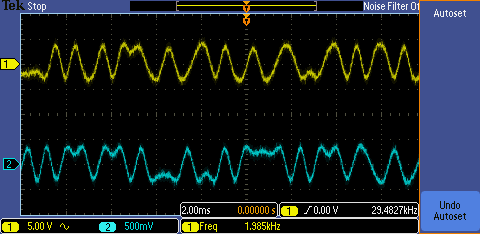
\includegraphics[width=0.65\textwidth]{img/task_a_oscilloscope.png}
    \caption{In-phase and Quadrature component.}
  \end{center}
\end{figure}

\begin{figure}[h]
  \begin{center}
    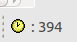
\includegraphics[width=0.65\textwidth]{img/task_a_profile.png}
    \caption{In-phase and Quadrature profile.}
  \end{center}
\end{figure}

\pagebreak
\textbf{Task b)}

\begin{figure}[h]
  \begin{center}
    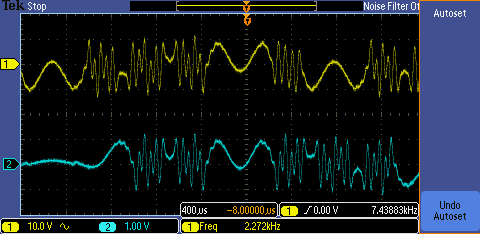
\includegraphics[width=0.65\textwidth]{img/task_b_oscilloscope.png}
    \caption{In-phase and Quadrature component of PN sequence.}
  \end{center}
\end{figure}

\begin{figure}[h]
  \begin{center}
    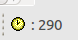
\includegraphics[width=0.65\textwidth]{img/task_b_profile.png}
    \caption{In-phase and Quadrature profile of PN sequence.}
  \end{center}
\end{figure}

\pagebreak
\textbf{Task c)}

\begin{figure}[h]
  \begin{center}
    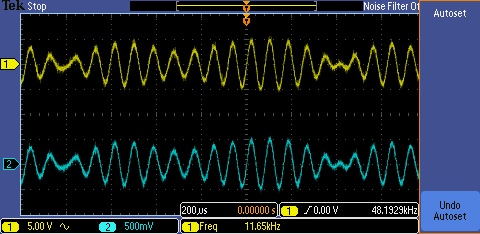
\includegraphics[width=0.65\textwidth]{img/task_c_oscilloscope.png}
    \caption{In-phase and Quadrature component of optimized pulse shape.}
  \end{center}
\end{figure}

\begin{figure}[h]
  \begin{center}
    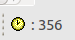
\includegraphics[width=0.65\textwidth]{img/task_c_profile.png}
    \caption{In-phase and Quadrature profile of optimized pulse shape.}
  \end{center}
\end{figure}

\pagebreak
\textbf{Task d)}

\begin{figure}[h]
  \begin{center}
    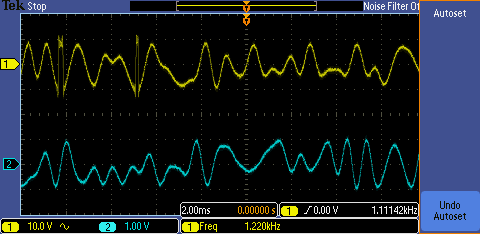
\includegraphics[width=0.65\textwidth]{img/task_d_oscilloscope.png}
    \caption{In-phase and Quadrature component of 16-QAM.}
  \end{center}
\end{figure}

\begin{figure}[h]
  \begin{center}
    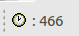
\includegraphics[width=0.65\textwidth]{img/task_d_profile.png}
    \caption{In-phase and Quadrature component of 16-QAM PN sequence.}
  \end{center}
\end{figure}

\pagebreak
\textbf{Code: 16-QAM}

\begin{verbatim}

	// left (quadrature), right (in-phase)
	const float QPSK_LUT[16][2] = {
	{     -3 * QPSK_SCALE,  -3 * QPSK_SCALE}, /* QPSK_LUT[0]  */
	{     -3 * QPSK_SCALE, -1 * QPSK_SCALE}, /* QPSK_LUT[1]  */
	{    -3 * QPSK_SCALE,  3 * QPSK_SCALE}, /* QPSK_LUT[2]  */
	{    -3 * QPSK_SCALE,  1 * QPSK_SCALE}, /* QPSK_LUT[3]  */
	{    -1 * QPSK_SCALE, -3 * QPSK_SCALE}, /* QPSK_LUT[4]  */
	{    -1 * QPSK_SCALE, -1 * QPSK_SCALE}, /* QPSK_LUT[5]  */
	{    -1 * QPSK_SCALE,  3 * QPSK_SCALE}, /* QPSK_LUT[6]  */
	{    -1 * QPSK_SCALE,  1 * QPSK_SCALE}, /* QPSK_LUT[7]  */
	{     3 * QPSK_SCALE, -3 * QPSK_SCALE}, /* QPSK_LUT[8]  */
	{     3 * QPSK_SCALE, -1 * QPSK_SCALE}, /* QPSK_LUT[9]  */
	{     3 * QPSK_SCALE,  3 * QPSK_SCALE}, /* QPSK_LUT[10]  */
	{     3 * QPSK_SCALE,  1 * QPSK_SCALE}, /* QPSK_LUT[11]  */
	{     1 * QPSK_SCALE, -3 * QPSK_SCALE}, /* QPSK_LUT[12]  */
	{     1 * QPSK_SCALE, -1 * QPSK_SCALE}, /* QPSK_LUT[13]  */
	{     1 * QPSK_SCALE,  3 * QPSK_SCALE}, /* QPSK_LUT[14]  */
	{     1 * QPSK_SCALE, -1 * QPSK_SCALE}, /* QPSK_LUT[15]  */
	};

	/************************************************************/
	// I added my impulse modulated QPSK routine here
	if (counter == 0) {
		symbol = rand() & 0xF;

		xI[0]  = QPSK_LUT[symbol][RIGHT];  
		xQ[0]  = QPSK_LUT[symbol][ LEFT];   
	}

	// perform impulse modulation based on the FIR filter, B[N]
	yI = 0;
	yQ = 0;

	for (i = 0; i < span; i++) {
		// perform the "I" dot-product
		yI += xI[i]*pulse[counter + samplesPerSymbol*i];	

		// perform the "Q" dot-product
		yQ += xQ[i]*pulse[counter + samplesPerSymbol*i];	
	}

	if (counter >= (samplesPerSymbol - 1)) {
		counter = -1; 

		/* shift xI[] and xQ[] in preparation to receive the next input */
		for (i = 5; i > 0; i--) {
			// setup xI[] for the next input value
			xI[i] = xI[i-1];  

			// setup xQ[] for the next input value
			xQ[i] = xQ[i-1];  
		}
	}

	counter++;

	output = output_gain*(yI*cosine[counter & 3] - yQ*sine[counter & 3]);
\end{verbatim}

\pagebreak
\textbf{Task e)}

\begin{figure}[h]
  \begin{center}
    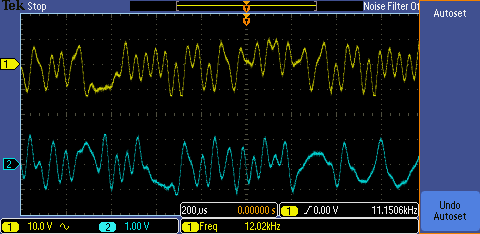
\includegraphics[width=0.65\textwidth]{img/task_e_oscilloscope.png}
    \caption{In-phase and Quadrature component of PN sequence.}
  \end{center}
\end{figure}

\begin{figure}[h]
  \begin{center}
    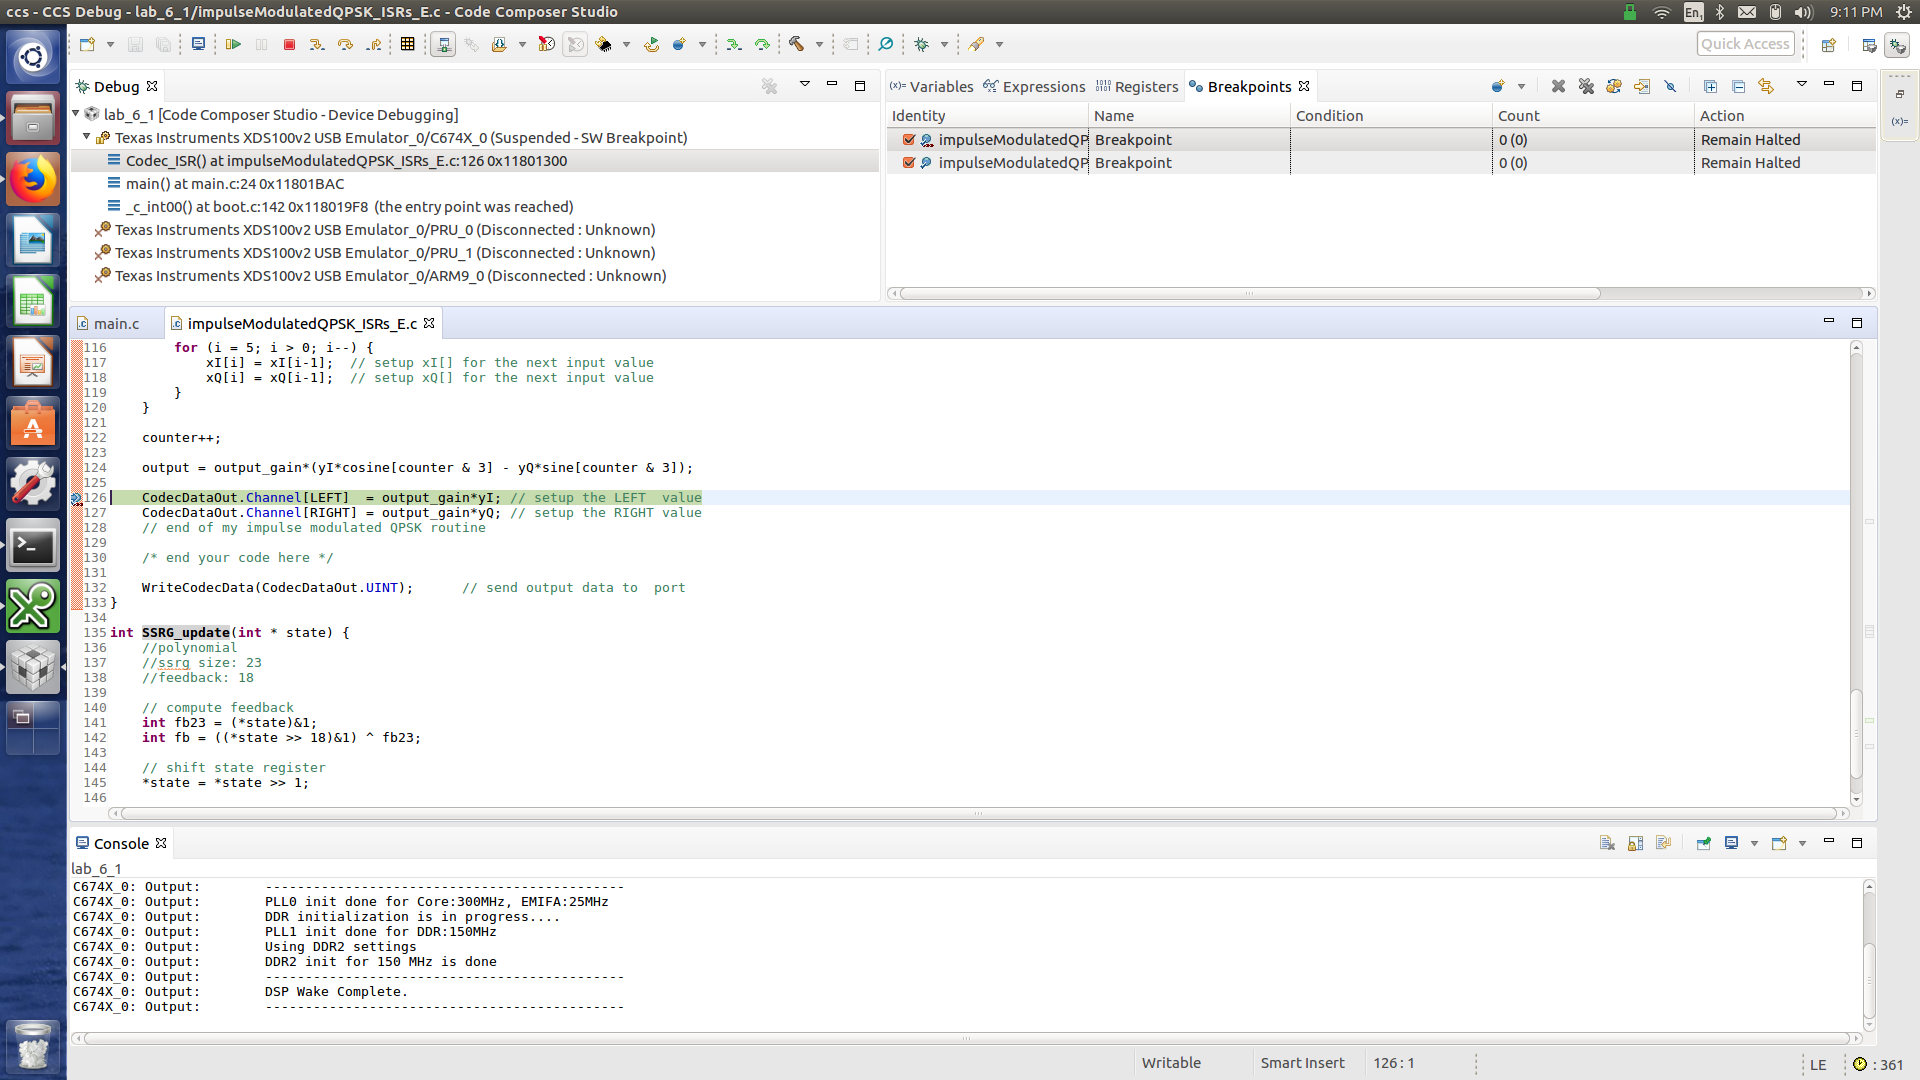
\includegraphics[width=0.65\textwidth]{img/task_e_profile.png}
    \caption{In-phase and Quadrature component of PN sequence.}
  \end{center}
\end{figure}

\pagebreak
\textbf{Code: 16-QAM with PN sequence}

\begin{verbatim}

	// left (quadrature), right (in-phase)
	const float QPSK_LUT[16][2] = {
	{     -3 * QPSK_SCALE,  -3 * QPSK_SCALE}, /* QPSK_LUT[0]  */
	{     -3 * QPSK_SCALE, -1 * QPSK_SCALE}, /* QPSK_LUT[1]  */
	{    -3 * QPSK_SCALE,  3 * QPSK_SCALE}, /* QPSK_LUT[2]  */
	{    -3 * QPSK_SCALE,  1 * QPSK_SCALE}, /* QPSK_LUT[3]  */
	{    -1 * QPSK_SCALE, -3 * QPSK_SCALE}, /* QPSK_LUT[4]  */
	{    -1 * QPSK_SCALE, -1 * QPSK_SCALE}, /* QPSK_LUT[5]  */
	{    -1 * QPSK_SCALE,  3 * QPSK_SCALE}, /* QPSK_LUT[6]  */
	{    -1 * QPSK_SCALE,  1 * QPSK_SCALE}, /* QPSK_LUT[7]  */
	{     3 * QPSK_SCALE, -3 * QPSK_SCALE}, /* QPSK_LUT[8]  */
	{     3 * QPSK_SCALE, -1 * QPSK_SCALE}, /* QPSK_LUT[9]  */
	{     3 * QPSK_SCALE,  3 * QPSK_SCALE}, /* QPSK_LUT[10]  */
	{     3 * QPSK_SCALE,  1 * QPSK_SCALE}, /* QPSK_LUT[11]  */
	{     1 * QPSK_SCALE, -3 * QPSK_SCALE}, /* QPSK_LUT[12]  */
	{     1 * QPSK_SCALE, -1 * QPSK_SCALE}, /* QPSK_LUT[13]  */
	{     1 * QPSK_SCALE,  3 * QPSK_SCALE}, /* QPSK_LUT[14]  */
	{     1 * QPSK_SCALE, -1 * QPSK_SCALE}, /* QPSK_LUT[15]  */
	};

	/************************************************************/
	// I added my impulse modulated QPSK routine here
	if (counter == 0) {
		/* generate 2 random bits */
		symbol = SSRG_update(&SSRG_state); 
		symbol = (symbol << 1) + SSRG_update(&SSRG_state);
		symbol = (symbol << 1) + SSRG_update(&SSRG_state);
		symbol = (symbol << 1) + SSRG_update(&SSRG_state);

		xI[0]  = QPSK_LUT[symbol][RIGHT];  
		xQ[0]  = QPSK_LUT[symbol][ LEFT];   
	}

	// perform impulse modulation based on the FIR filter, B[N]
	yI = 0;
	yQ = 0;

	for (i = 0; i < span; i++) {
		// perform the "I" dot-product
		yI += xI[i]*pulse[counter + samplesPerSymbol*i];	

		// perform the "Q" dot-product
		yQ += xQ[i]*pulse[counter + samplesPerSymbol*i];	
	}

	if (counter >= (samplesPerSymbol - 1)) {
		counter = -1; 

		/* shift xI[] and xQ[] in preparation to receive the next input */
		for (i = 5; i > 0; i--) {
			// setup xI[] for the next input value
			xI[i] = xI[i-1];  

			// setup xQ[] for the next input value
			xQ[i] = xQ[i-1];  
		}
	}

	counter++;

	output = output_gain*(yI*cosine[counter & 3] - yQ*sine[counter & 3]);
\end{verbatim}

\pagebreak
\textbf{Task 2b)}

\begin{figure}[h]
  \begin{center}
    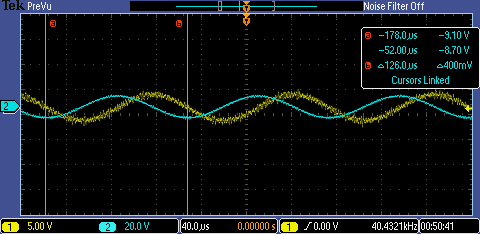
\includegraphics[width=0.65\textwidth]{img/task_2_b_oscilloscope.png}
    \caption{8kHz carrier wave.}
  \end{center}
\end{figure}

\begin{figure}[h]
  \begin{center}
    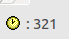
\includegraphics[width=0.65\textwidth]{img/task_2_b_profile.png}
    \caption{8kHz carrier wave profile.}
  \end{center}
\end{figure}

\pagebreak
\textbf{Task 2c)}

\begin{figure}[h]
  \begin{center}
    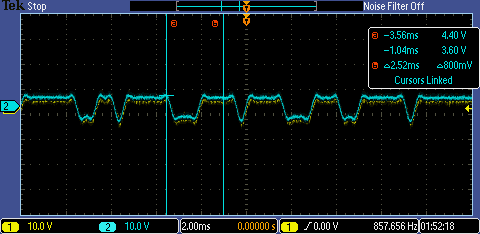
\includegraphics[width=0.65\textwidth]{img/task_2_c_oscilloscope.png}
    \caption{Demodulated in-phase component.}
  \end{center}
\end{figure}

\begin{figure}[h]
  \begin{center}
    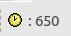
\includegraphics[width=0.65\textwidth]{img/task_2_c_profile.png}
    \caption{Demodulated in-phase profile.}
  \end{center}
\end{figure}

\pagebreak
\textbf{Task 2d)}

\begin{figure}[h]
  \begin{center}
    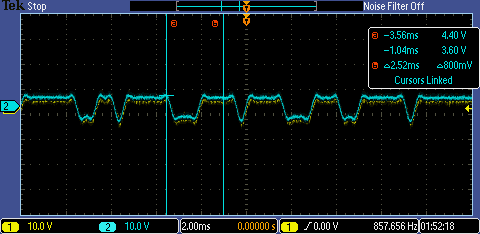
\includegraphics[width=0.65\textwidth]{img/task_2_c_oscilloscope.png}
    \caption{Demodulated quadrature component.}
  \end{center}
\end{figure}

\begin{figure}[h]
  \begin{center}
    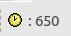
\includegraphics[width=0.65\textwidth]{img/task_2_c_profile.png}
    \caption{Demodulated quadrature profile.}
  \end{center}
\end{figure}

\pagebreak
\textbf{Code: Reciever Demodulation}

\begin{verbatim}
	// I added my impulse modulated QPSK routine here
	if (counter == 0) {
		/* generate 2 random bits */
		symbol = SSRG_update(&SSRG_state); 
		symbol = (symbol << 1) + SSRG_update(&SSRG_state);

		xI[0]  = QPSK_LUT[symbol][RIGHT];  
		xQ[0]  = QPSK_LUT[symbol][ LEFT];   
	}

	// perform impulse modulation based on the FIR filter, B[N]
	yI = 0;
	yQ = 0;

	for (i = 0; i < span; i++) {
		// perform the "I" dot-product
		yI += xI[i]*pulse[counter + samplesPerSymbol*i];	

		// perform the "Q" dot-product
		yQ += xQ[i]*pulse[counter + samplesPerSymbol*i];	
	}

	if (counter >= (samplesPerSymbol - 1)) {
		counter = -1; 

		/* shift xI[] and xQ[] in preparation to receive the next input */
		for (i = 5; i > 0; i--) {
			// setup xI[] for the next input value
			xI[i] = xI[i-1];  

			// setup xQ[] for the next input value
			xQ[i] = xQ[i-1];  
		}
	}

	counter++;
	carrier_index = (carrier_index + 1) % 6;

	output = output_gain*(yI*cosine[carrier_index] - yQ*sine[carrier_index]);
	// end of my impulse modulated QPSK routine

	//demodulate in-phase and quadrature
  float demod_inphase = 2*output*cosine[carrier_index];
  float demod_quad = -2*output*sine[carrier_index];

  //LPF
  biquad_x_inphase[0][0] = demod_inphase;
  biquad_x_quad[0][0] = demod_quad;

  float output_inphase = G[0] * biquad_inphase(0, biquad_x_inphase[0][0]);
  float output_quad = G[0] * biquad_quadrature(0, biquad_x_quad[0][0]);
\end{verbatim}

%----------------------------------------------------------------------------------------
%	SECTION 4
%----------------------------------------------------------------------------------------

\section{Discussion}

\subsection{Part 1: Understanding QAM Transmission}

\subsubsection{Task A + B: QAM Transmitter Design}

\subsubsection{Task C: Optimized Pulse Shaping for QAM Transmitter}

\subsubsection{Task D + E: Modifications for 16-QAM}

\subsection{Part 2: Understanding QAM Demodulation}

\subsubsection{Task A + B: Transmitter Modifications for QAM Demodulation}

\subsubsection{Task C + D: QAM Receiver Design}


%----------------------------------------------------------------------------------------
%	SECTION 5
%----------------------------------------------------------------------------------------

\section{Answers to questions}

\begin{enumerate}
  \begin{item}
    Explain why we changed the carrier frequency to properly simulate the receiver. 

  \textbf{Answer:}
    The sampling rate of the DSP board is set to 48kHz so the maximum frequency that we can represent is 24kHz.
    If we kept the the frequency of the carrier at 12kHz, then when we demodulated we would have a sinusoid alias to DC
    because we would get the original baseband signal plus a sinusoid with twice the carrier frequency.
  \end{item}

  \begin{item}
    Explain your choice of cutoff frequency for the demodulation filter.

  \textbf{Answer:}
    The cutoff must be equal to the bandwidth of the baseband signal, but less than twice the carrier frequency.
  \end{item}

  \begin{item}
    The QAM signal can be viewed as the sum of two PAM signals that each have been modulated by a carrier. How is the bandwidth of the QAM signal related to the bandwidth of its two (carrier-modulated) PAM components?

  \textbf{Answer:}
    QAM encodes information in both the amplitude and phase of the carrier, where as PAM only encodes information in the amplitude of the carrier.
    So PAM takes twice the bandwidth of QAM.

  \end{item}
\end{enumerate}

\end{document}
